\chapter{Flores, frutos y semillas}\label{ch:g3:flowers-fruits-seeds}

En abril el cerezo está blanco de \omterm{def:g3:flowers-fruits-seeds:parts}{flores}; en junio está cargado de
cerezas. ¿Adónde se fueron las \omterm{def:g3:flowers-fruits-seeds:parts}{flores} --- y de dónde salió la fruta?
La respuesta es una de las transformaciones más bonitas del mundo
vivo: la \omterm{def:g3:flowers-fruits-seeds:parts}{flor} no desaparece, se \emph{convierte} en el \omterm{prop:g3:flowers-fruits-seeds:transform}{fruto}.

\section{Mirar dentro de una flor}

\begin{definition}[Las partes de una flor]\label{def:g3:flowers-fruits-seeds:parts}
Una \emph{flor}\index{flor} es la parte de la \omterm{def:g1:plants-around-us:plant}{planta} que hará las
\omterm{prop:g3:flowers-fruits-seeds:transform}{semillas}. De fuera hacia dentro:
\begin{enumerate}
  \item los \emph{pétalos}\index{pétalo}, de colores y con olor, que
        atraen a los \omterm{prop:g3:sorting-living-things:groups}{insectos} que la visitan;
  \item los \emph{estambres}\index{estambre}, tallitos finos
        espolvoreados de \emph{polen}\index{polen}, un polvo amarillo
        muy fino;
  \item en el mismo centro, el \emph{pistilo}\index{pistilo}, una
        botellita; en su fondo están las futuras \omterm{prop:g3:flowers-fruits-seeds:transform}{semillas} de la flor.
\end{enumerate}
\end{definition}

\begin{omfigure}
\begin{tikzpicture}
  \node[anchor=south west, inner sep=0] (img) at (0,0)
    {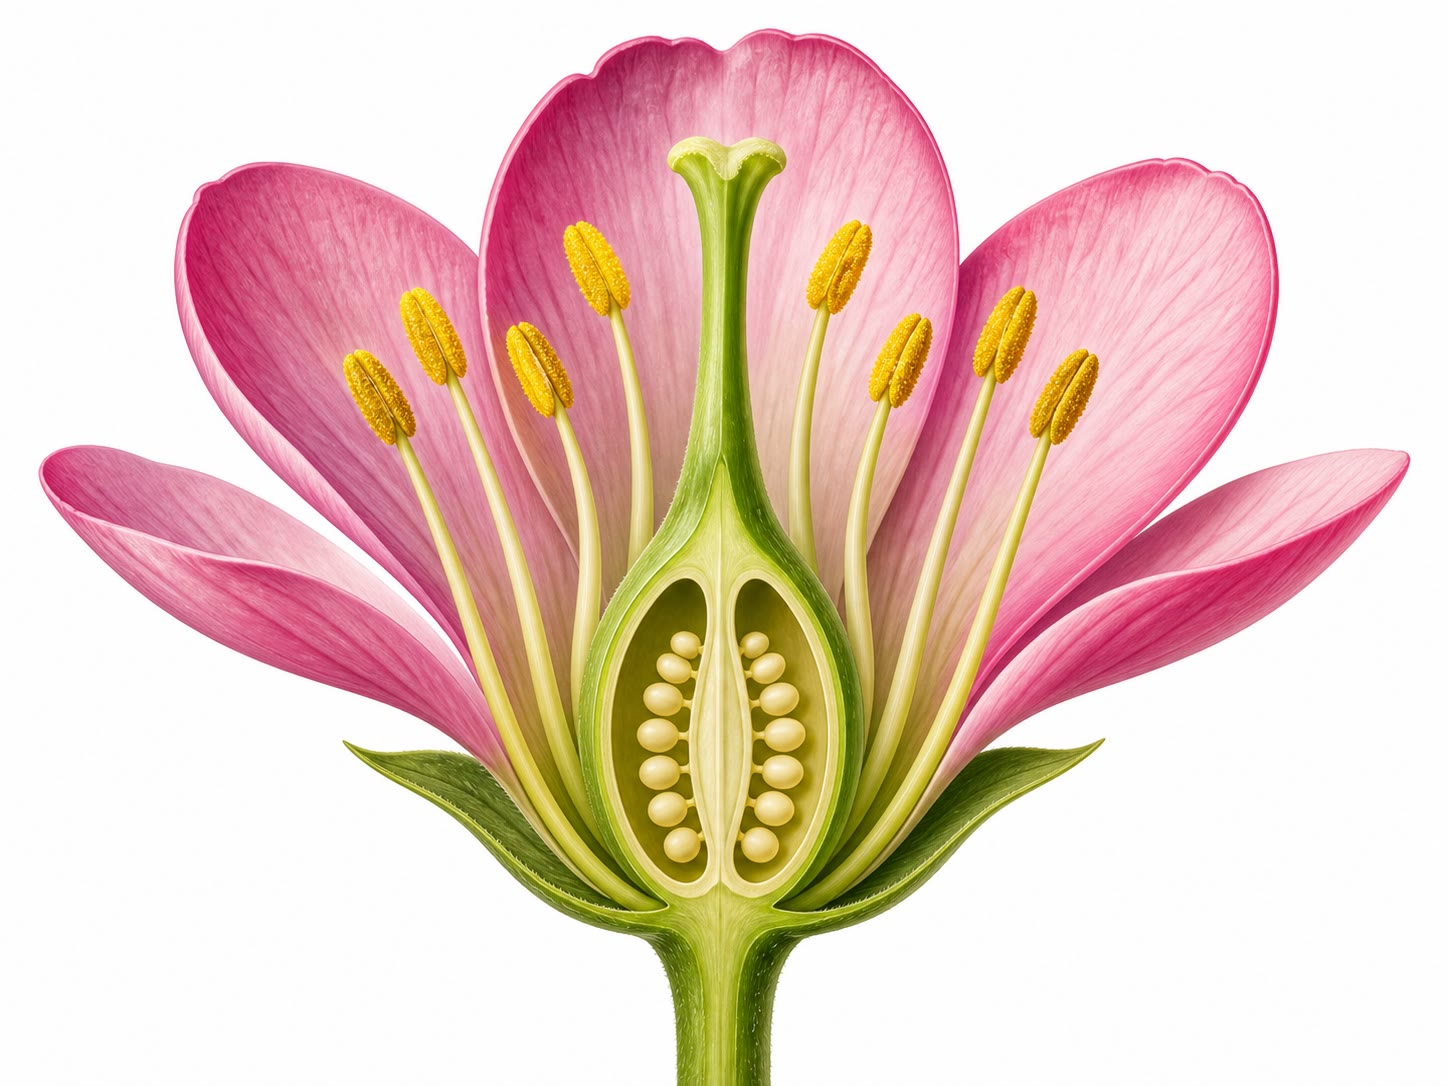
\includegraphics[width=0.6\linewidth]{images/book1/ai/fig-flower-cutaway.jpg}};
  \begin{scope}[x={(img.south east)}, y={(img.north west)},
      every node/.style={font=\small}]
    \draw[omDef, thick] (0.82,0.80) -- (0.93,0.90) node[above] {pétalo};
    \draw[omDef, thick] (0.72,0.68) -- (1.03,0.66)
      node[right, align=left] {estambre, espolvoreado\\ de polen};
    \draw[omDef, thick] (0.56,0.36) -- (1.03,0.34)
      node[right, align=left] {pistilo: dentro están\\ las futuras semillas};
    \draw[omDef, thick] (0.505,0.05) -- (0.66,0.04) node[right] {tallo};
  \end{scope}
\end{tikzpicture}

{\small Una \omterm{def:g3:flowers-fruits-seeds:parts}{flor} por dentro, cortada por la mitad: \omterm{def:g3:flowers-fruits-seeds:parts}{pétalos} alrededor,
\omterm{def:g3:flowers-fruits-seeds:parts}{estambres} con \omterm{def:g3:flowers-fruits-seeds:parts}{polen} y el \omterm{def:g3:flowers-fruits-seeds:parts}{pistilo} en el centro con las futuras \omterm{prop:g3:flowers-fruits-seeds:transform}{semillas}.}
\end{omfigure}

\begin{example}[Diseccionar un tulipán]\label{ex:g3:flowers-fruits-seeds:tulip}
Abre con cuidado un tulipán marchito, \omterm{def:g3:flowers-fruits-seeds:parts}{pétalo} a \omterm{def:g3:flowers-fruits-seeds:parts}{pétalo}. Dentro están
los \omterm{def:g3:flowers-fruits-seeds:parts}{estambres} --- pasa uno por el dedo y deja polvo amarillo de \omterm{def:g3:flowers-fruits-seeds:parts}{polen}
--- y en el centro el \omterm{def:g3:flowers-fruits-seeds:parts}{pistilo} verde y gordo. Corta el \omterm{def:g3:flowers-fruits-seeds:parts}{pistilo} de
través (con un cuchillo y con una persona mayor) y ahí están: filas de
futuras \omterm{prop:g3:flowers-fruits-seeds:transform}{semillas} pálidas y diminutas.
\end{example}

\section{De la flor al fruto}

\begin{proposition}[Polinización y después transformación]\label{prop:g3:flowers-fruits-seeds:transform}
Para que empiece la transformación, el \omterm{def:g3:flowers-fruits-seeds:parts}{polen} tiene que llegar al
\omterm{def:g3:flowers-fruits-seeds:parts}{pistilo} --- ese paso es la
\emph{polinización}\index{polinización}. Las abejas y otros \omterm{prop:g3:sorting-living-things:groups}{insectos}
hacen casi todo el transporte, espolvoreados de \omterm{def:g3:flowers-fruits-seeds:parts}{polen} mientras beben
de \omterm{def:g3:flowers-fruits-seeds:parts}{flor} en \omterm{def:g3:flowers-fruits-seeds:parts}{flor}; el viento hace una parte. Después de la polinización:
\begin{itemize}
  \item los \omterm{def:g3:flowers-fruits-seeds:parts}{pétalos} y los \omterm{def:g3:flowers-fruits-seeds:parts}{estambres}, con su trabajo hecho, se
        marchitan y caen;
  \item el \omterm{def:g3:flowers-fruits-seeds:parts}{pistilo} se hincha y se convierte en el
        \emph{fruto}\index{fruto};
  \item las futuras \omterm{prop:g3:flowers-fruits-seeds:transform}{semillas} de dentro se convierten en las
        \emph{semillas}\index{semilla}.
\end{itemize}
Un \omterm{prop:g3:flowers-fruits-seeds:transform}{fruto} es un \omterm{def:g3:flowers-fruits-seeds:parts}{pistilo} transformado, y todo \omterm{prop:g3:flowers-fruits-seeds:transform}{fruto} verdadero lleva
\omterm{prop:g3:flowers-fruits-seeds:transform}{semillas}.
\end{proposition}
\admitted

\begin{example}[Ver cómo ocurre una cereza]\label{ex:g3:flowers-fruits-seeds:cherry}
Sigue una sola \omterm{def:g3:flowers-fruits-seeds:parts}{flor} de cerezo. Abril: \omterm{def:g3:flowers-fruits-seeds:parts}{pétalos} blancos, abejas
zumbando. Mayo: nieve de \omterm{def:g3:flowers-fruits-seeds:parts}{pétalos} que caen; donde estaba cada \omterm{def:g3:flowers-fruits-seeds:parts}{flor}, una
bolita verde --- el \omterm{def:g3:flowers-fruits-seeds:parts}{pistilo} que se hincha. Junio: la bolita ya roja y
dulce --- una cereza, con el hueso (su \omterm{def:g2:from-seed-to-plant:seed}{semilla}) dentro. La \omterm{def:g3:flowers-fruits-seeds:parts}{flor} no se
cayó; solo se cayeron sus \omterm{def:g3:flowers-fruits-seeds:parts}{pétalos}.
\end{example}

\begin{remark}[Sin abejas no hay cerezas]\label{rem:g3:flowers-fruits-seeds:bees}
Los cultivadores de cerezas reciben con gusto las colmenas de los
apicultores en sus huertos --- sin las visitas de los \omterm{prop:g3:sorting-living-things:groups}{insectos}, casi
todas las \omterm{def:g3:flowers-fruits-seeds:parts}{flores} se quedarían sin polinizar y caerían sin llegar a ser
\omterm{prop:g3:flowers-fruits-seeds:transform}{fruto}. La abeja no le roba nada a la \omterm{def:g3:flowers-fruits-seeds:parts}{flor}; la \omterm{def:g3:flowers-fruits-seeds:parts}{flor} y la abeja se
alimentan mutuamente: néctar para la abeja, reparto de \omterm{def:g3:flowers-fruits-seeds:parts}{polen} para la
\omterm{def:g1:plants-around-us:plant}{planta}.
\end{remark}

\begin{omfigure}
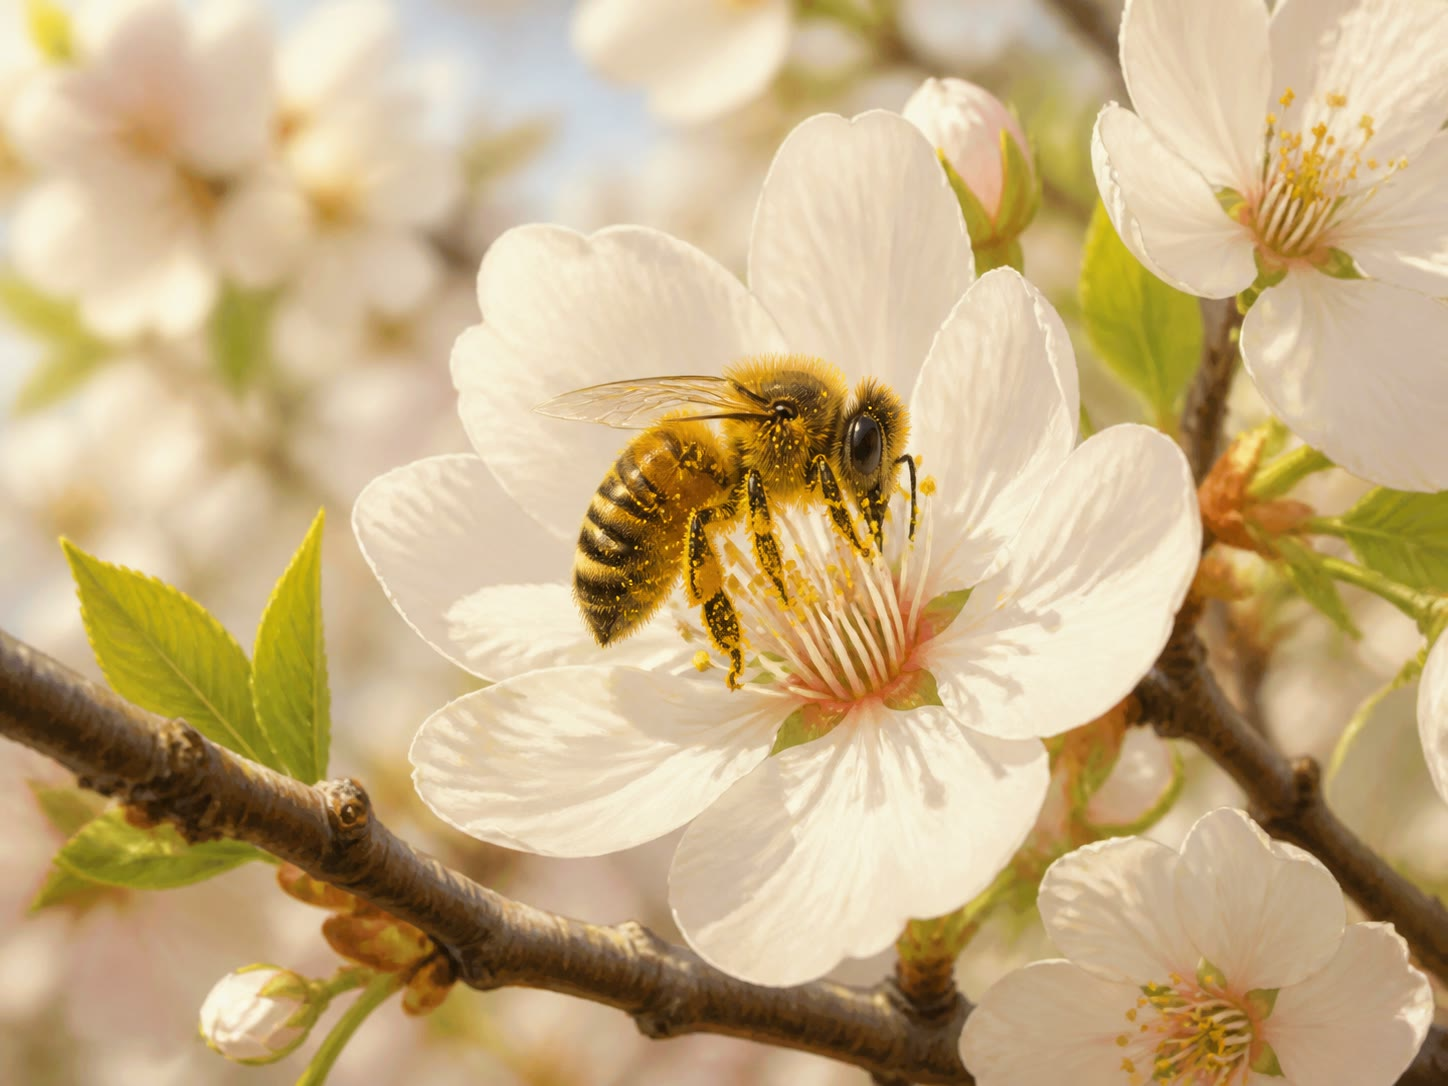
\includegraphics[width=0.58\linewidth]{images/book1/ai/g3-flowers-bee.jpg}

{\small Polinización en marcha: una abeja en el fondo de una \omterm{def:g3:flowers-fruits-seeds:parts}{flor} de
cerezo, cubierta del \omterm{def:g3:flowers-fruits-seeds:parts}{polen} que llevará a la \omterm{def:g3:flowers-fruits-seeds:parts}{flor} siguiente.}
\end{omfigure}

\section{¿Fruto o no fruto?}

\begin{method}[La prueba de la semilla]\label{met:g3:flowers-fruits-seeds:test}
Para decidir si algo de la frutería es un \omterm{prop:g3:flowers-fruits-seeds:transform}{fruto} en el sentido del
biólogo:
\begin{enumerate}
  \item ábrelo;
  \item busca \omterm{prop:g3:flowers-fruits-seeds:transform}{semillas} (o un hueso, que es una \omterm{def:g2:from-seed-to-plant:seed}{semilla} dentro de una
        cáscara dura);
  \item si hay \omterm{prop:g3:flowers-fruits-seeds:transform}{semillas} dentro --- creció del \omterm{def:g3:flowers-fruits-seeds:parts}{pistilo} de una \omterm{def:g3:flowers-fruits-seeds:parts}{flor}: es
        un \omterm{prop:g3:flowers-fruits-seeds:transform}{fruto}. Si no hay ninguna --- es otra parte de la \omterm{def:g1:plants-around-us:plant}{planta}:
        \omterm{def:g1:plants-around-us:parts}{raíz}, \omterm{def:g1:plants-around-us:parts}{tallo} u \omterm{def:g1:plants-around-us:parts}{hoja}.
\end{enumerate}
\end{method}

\begin{example}[Sorpresas en la frutería]\label{ex:g3:flowers-fruits-seeds:surprise}
La prueba de la \omterm{def:g2:from-seed-to-plant:seed}{semilla} da sorpresas. El tomate: lleno de \omterm{prop:g3:flowers-fruits-seeds:transform}{semillas} ---
un \omterm{prop:g3:flowers-fruits-seeds:transform}{fruto}, diga lo que diga la ensaladera. El pepino y el calabacín:
\omterm{prop:g3:flowers-fruits-seeds:transform}{semillas} --- \omterm{prop:g3:flowers-fruits-seeds:transform}{frutos}. La vaina de judía verde: \omterm{prop:g3:flowers-fruits-seeds:transform}{semillas} en fila --- un
\omterm{prop:g3:flowers-fruits-seeds:transform}{fruto}. La zanahoria: sin \omterm{prop:g3:flowers-fruits-seeds:transform}{semillas} --- una \omterm{def:g1:plants-around-us:parts}{raíz} (el
\cref{exo:g1:plants-around-us:10} lo adivinó). La lechuga: sin
\omterm{prop:g3:flowers-fruits-seeds:transform}{semillas} --- \omterm{def:g1:plants-around-us:parts}{hojas}. La patata: sin \omterm{prop:g3:flowers-fruits-seeds:transform}{semillas} --- un \omterm{def:g1:plants-around-us:parts}{tallo} subterráneo
engordado.
\end{example}

\begin{remark}[Palabras de cocina, palabras de ciencia]\label{rem:g3:flowers-fruits-seeds:words}
En la cocina, ``fruta'' quiere decir dulce y ``verdura'' quiere decir
salado --- útil para planear el postre, inútil para la \omterm{def:g1:living-or-not:living}{biología}. La
palabra del biólogo sigue la prueba de la \omterm{def:g2:from-seed-to-plant:seed}{semilla}. Los dos
vocabularios están bien, siempre que sepas cuál estás hablando.
\end{remark}

\section{Ejercicios}

\begin{exercise}[$\star$]\label{exo:g3:flowers-fruits-seeds:1}
Nombra las partes de una \omterm{def:g3:flowers-fruits-seeds:parts}{flor} de fuera hacia dentro, con la tarea de
cada parte.
\end{exercise}

\begin{exercise}[$\star$]\label{exo:g3:flowers-fruits-seeds:2}
¿Qué es el \omterm{def:g3:flowers-fruits-seeds:parts}{polen} y dónde se encuentra? ¿Qué es la polinización?
\end{exercise}

\begin{exercise}[$\star$]\label{exo:g3:flowers-fruits-seeds:3}
Después de la polinización, ¿en qué se convierten: (a) los \omterm{def:g3:flowers-fruits-seeds:parts}{pétalos}?
(b) el \omterm{def:g3:flowers-fruits-seeds:parts}{pistilo}? (c) las futuras \omterm{prop:g3:flowers-fruits-seeds:transform}{semillas} de dentro?
\end{exercise}

\begin{exercise}[$\star$]\label{exo:g3:flowers-fruits-seeds:4}
Vuelve a contar la historia de una cereza, de la \omterm{def:g3:flowers-fruits-seeds:parts}{flor} blanca al \omterm{prop:g3:flowers-fruits-seeds:transform}{fruto}
rojo, en tres pasos con fecha.
\end{exercise}

\begin{exercise}[$\star$]\label{exo:g3:flowers-fruits-seeds:5}
¿Por qué reciben con gusto los cultivadores de cerezas las colmenas en el huerto?
\end{exercise}

\begin{exercise}[$\star$]\label{exo:g3:flowers-fruits-seeds:6}
Enuncia la prueba de la \omterm{def:g2:from-seed-to-plant:seed}{semilla} y aplícasela al tomate y a la zanahoria.
\end{exercise}

\begin{exercise}[$\star$]\label{exo:g3:flowers-fruits-seeds:7}
¿\omterm{prop:g3:flowers-fruits-seeds:transform}{Fruto} o no, según la prueba de la \omterm{def:g2:from-seed-to-plant:seed}{semilla}: el pepino, la lechuga, la
vaina de judía verde, la patata?
\end{exercise}

\begin{exercise}[$\star$]\label{exo:g3:flowers-fruits-seeds:8}
Pruébalo: en casa, abre tres cosas de la cocina y pásale a cada una la
prueba de la \omterm{def:g2:from-seed-to-plant:seed}{semilla}. ¿Cuál te sorprendió?
\end{exercise}

\begin{exercise}[$\star\star$]\label{exo:g3:flowers-fruits-seeds:9}
Una helada tardía mata en abril todas las \omterm{def:g3:flowers-fruits-seeds:parts}{flores} del ciruelo. ¿Cuál
será la cosecha de junio y por qué? Usa la
\cref{prop:g3:flowers-fruits-seeds:transform}.
\end{exercise}

\begin{exercise}[$\star\star$]\label{exo:g3:flowers-fruits-seeds:10}
``La manzana crece para que tengamos algo rico que comer''. ¿Para qué
sirve de verdad la manzana desde el punto de vista del manzano? ¿Qué
hay en su corazón y en qué se podría convertir cada una de esas cosas?
(Acuérdate del \cref{ch:g2:from-seed-to-plant}.)
\end{exercise}
